\section{Introduction}
Networks of small interlocking pods appear as a common thread throughout
successful large-scale collaborations.
However, it remains unclear whether that network structure plays a causal role
in the success of those collaborations,
and whether the specific structural properties of that interlocking network matter.
Observational study suggests a correlation between properties such as degree,
structural efficiency, and structural inequality and the performance/productivity
of collaborations \cite{platt_network_2018}.
Numerical simulation suggests a causal relationship in a simplified theoretical
setting (Chapter \ref{chap:abm}).
To bridge these two findings,
this chapter presents the results of an online experiment studying the role of network deliberation in the evolution of group preferences.

Collaboration and collective action allow groups of individuals to manage shared resources and combine efforts towards common goals, but also introduce the problem of governance and collective decision-making.
While collective governance of common resources is a historically hard problem, Ostrom described principles seen in successful systems \cite{ostrom_collective_2000}.
More recently, the proliferation of inexpensive point-to-point global communication via the internet has enabled a number of successful large-scale collaborations and movements, including free/open-source software \cite{benkler_coases_2002, coleman_coding_2012, raymond_cathedral_1999}, Wikipedia \cite{keegan_evolution_2017, benkler_coases_2002, giles_internet_2005}, and social movements \cite{tufekci_twitter_2017, gonzalez-bailon_networked_2016}.

Scholars of democracy commonly describe governance systems in terms of two axes: representation and argumentation \cite{ackerman_deliberation_2002, gonzalez-bailon_networked_2016}. Here, {\em representation} refers to how many people participate in decision-making, while {\em argumentation} refers to the amount of discourse between the decision-makers.
While both can improve governance, they are difficult to achieve simultaneously \cite{gentry_consensus_1982, freeman_tyranny_1972} and tradeoffs can be made to favor one over the other, as in voting (high representation, low argumentation) and representative democracy (low representation, high argumentation).

We focus on deliberation due to fundamental limitations of voting.
Results from social choice theory showt that any ranked-choice voting system is subject to limitations such as the Condorcet Paradox \cite{condorcet_essay_1785} and Arrow's Impossibility Theorem \cite{arrow_social_2012}.
Deliberation offers one way to avoid these limitations by changing individual preferences \cite{ackerman_deliberation_2002}.
The success of deliberation at generating consensus has been attributed to its ability to identify and resolve conflict \cite{gentry_consensus_1982}.
However, deliberation also carries risks, such as the posibility of pushing individuals towards extreme and polarized preferences \cite{schkade_what_2007}.

In any sufficiently large group, it becomes unfeasible for all members to interact with each other.
Understanding collaboration in large groups thus requires attention to the network structure of who interacts with whom.
The field of social learning has studied both simple estimation tasks \cite{degroot_reaching_1974, golub_naive_2010} and more complex rugged-landscape optimization tasks \cite{lazer_network_2007, barkoczi_social_2016}.
Observational studies have been used to analyze the network structures of online collaborations \cite{gonzalez-bailon_networked_2016, platt_network_2018}.
Lab and field studies have also been used to study real-world collaborations on a small scale \cite{salehi_hive_2018, kearns_experiments_2012}.
As discussed in Chapter \ref{chap:abm}, the successful large-scale collaborations enabled by the internet often exhibit network sructures characterized by small, interlocking groups, reminiscent of interlocking directorates \cite{levine_study_1979} and interlocking publics \cite{habermas_structural_1991}.
In Chapter \ref{chap:abm}, we describe agent-based simulations showing that such network deliberation can improve performance on complex tasks when individuals exhibit strong social influence.dsd
Here, we expand on existing research by performing a controlled online experimental evaluation of network deliberation.
We use periodic polling to track preference evolution, allowing causal inference in a real-world setting.

While many studies have examined the role of network structure in collaboration, there has so far been little attention to the interlocking pod structure of network deliberation.
The closest we are aware of is the study of network rotation by Salehi \& Bernstein \cite{salehi_hive_2018}.
The present experiment goes beyond existing work primarily by tracking preferences throughout the experiment and by the use of a conventional single-group control condition.
We also describe multiple network deliberation topologies for achieving efficient or inefficient networks.
For the present study, we focus on an efficient topology.

The experiment described here focuses on several issues.
Based on observational and numerical findings that successful large-scale collaborations often exhibit network deliberation struture, we test the following hypothesis:
\begin{description}
\item[H1:] Network deliberation results in higher agreement among participants than single large-group deliberation.
\end{description}
We are also concerned with the dynamics of preference evolution under network deliberation, which may provide insight into possible mechanisms.
One such mechanism proposed in consensus decision-making literature is the ability to identify and resolve conflict.
We thus also seek to address two research questions:
\begin{description}
\item[RQ1:] How do preferences evolve throughout network deliberation?
\item[RQ2:] How effective is network deliberation at identifying and resolving conflict?
\end{description}

We find difference in preference evolution between network deliberation and conventional deliberation. Our primary contributions are:
\begin{itemize}
    \item We find experimental support for the hypothesis that network deliberation is better at facilitating agreement than conventional deliberation.
    \item We find evidence suggesting network deliberation can provide protection against information cascades.
    \item We find no evidence that network deliberation facilitates substantial conflict-resolution, but that it may provide protection against polarization.
\end{itemize}

We present relevant theory in Section \ref{sec:theory}.
We describe the experiment in Section \ref{sec:experiment} and present the results in Section \ref{sec:res}.
We discuss the results in Section \ref{sec:discussion} and conclude in Section \ref{sec:ch04conclusion}.

\section{Theory}
\label{sec:theory}
\subsection{Social Choice Theory}
Our analysis of preferences is foudned in the formalism of social choice theory \cite{arrow_social_2012, gaertner_primer_2009}.
In social choice theory, individual's {\em preferences} are represented by a ranked ordering of {\em alternatives} (e.g., proposals, candidates).
The set of preferences for all individuals in a group is called the {\em preference profile}.
A {\em social welfare function} can be applied to the profile to generate a {\em social preference}: an ordering of alternatives representing the preference of the group as a whole.
A {\em social choice function} represents a voting system: it selects a subset of winners from the available alternatives.

\subsection{Quantifying Agreement}

Social choice theory typically focuses on identifying and describing the limitations of specific voting systems.
Instead, we build on social choice theory to quantify the level of agreement in a group, based in individual profiles.

We use ranked-choice polls to construct preference profiles which are used to quantify agreement and conflict over the course of deliberation.
Within social choice theory, agreement can be defined by a {\em consensus class},
a set of preference profiles meeting one of several consensus criteria
\cite{elkind_rationalizations_2016}.
Examples include strong unanimity (of rank orders),
unanimity (of winners),
majority (existence of majority),
Condorcet (existence of Condorcet winner),
and transitivity (of social preference).
On the most restrictive end, in strong unanimity and unanimity,
all decision-makers prefer the same alternative.
In contrast, transitivity only requires that the social preferences induced by
individual preferences are transitive.
Distance-rationalizable voting systems are defined by projecting the preference
profile onto the nearest consensus profile according to a suitable distance.
For example, Dodgson's method \cite{dodgson_method_1876, brandt_computational_2012}
defines a distance based on swapping adjacent entries in individual preference profiles.
However, for most voting systems,
finding the consensus profile that minimizes distance is NP-Hard
\cite{elkind_rationalizations_2016}.
Social choice theory also provides measures of distances between two individual
preference rankings.
These measures can be extended to create measures of agreement for entire
preference profiles that can be calculated efficiently.

One possibility is to measure the distance from strong unanimity.
Any distance metric $\delta$ with a range of $[0,1]$ can be converted to a measure of correlation with range $[-1, 1]$ by taking $1 - 2\delta$.
One such measure is based on the Kendall tau metric, and the corresponding Kendall tau correlation \cite{kendall_new_1938}.
The Kendall tau metric is the fraction of pairwise contests that have different results between two profiles.
By averaging the corresponding correlation over all pairs of members, an overall measure of agreement can be calculated for the group.
While commonly used in social choice theory, the Kendall tau weights all contests equally, regardless of the ranks of the alteratives.
In practical settings with a small number of winners, the contests between highly-ranked alternatives are more consequential than those of low-ranked alternatives;
participants don't care if they disagree on the ordering of losing alternatives as long as they agree on which ones win and lose.
Various weighted extensions of the Kendall metric have been proposed \cite{shieh_weighted_1998, can_weighted_2014},
each with benefits and drawbacks.
We propose our own based on metric structure, uniqueness, and efficiency of calculation, which we describe below.

\subsubsection{Weighted Crossing Distance}
We propose the following weighted distance metric for preference rankings.
Given a set of $M$ alternatives, there are $M-1$ ways to divide an ordering into two nonempty sets of adjacent alternatives, i.e., a high set and a low set.
For a pair of preferences $p, q$, we define a length $M - 1$ {\em crossing vector} $v_m(p, q)$ to be equal to the number of alternatives in the highest $m$ positions of $p$ and not in the highest $m$ positions of $q$ (it is easily shown that this measure is symmetric in $p$ and $q$).
Informally, $v_m$ is the number of alternatives that cross place $m$.
Each element of $v_m$ is an integer in the range $[0, v_m^{\max}]$ dependent on the index:
\begin{equation}
    v_m^{\max} =
    \begin{cases}
    m & m \leq (M - 1) / 2 \\
    M - m & (M - 1) / 2 < m \leq M - 1.
    \end{cases}
\end{equation}
We construct the weighted crossing distance by taking a weighted sum over this vector.
There are many potential choices for weights.
We choose the weight of place $m$ to be equal to the highest total of all lower ranked places plus one.
Thus the weight at index $i = M - m$ (noting that low rank corresponds to high $m$) is given by:
\begin{equation}
    w_i = 1 + \sum_{k=1}^{i-1} w_k v_k^{\max}.
\end{equation}

\subsection{Quantifying Social Influence}

We are particularly interested in the role of social influence in preference evolution and require a formalism to quantify and analzye social influence.
If two individuals preferences become closer, can we say whether one influenced the other? And if so, can we say which influence which?
We cannot answer either question with certainty from preferences alone, but we can construct a reasonable proxy based on some simplifying assumptions.
Namely, we will construct measures of social influence based on the assumptions that:
\begin{itemize}
    \item The magnitude of an individual's change in preference increases with their susceptibility with social influence;
    \item The magnitude of an individual's change in preference increases with the magnitude of the distance between their preference and the influencing preference.
\end{itemize}
Thus, if the distance between the preferences of individuals $A$ and $B$ decreases, and the preference of $B$ changed more than the preference of $A$, we assume that individual $A$ influenced individual $B$.
We now describe two formal measures that use these assumptions to quantify how susceptible to influence and how potential influential an individual is.

\subsubsection{Conformity and Hipness}

Let $X$ be a set of alternatives (e.g., proposals or candidates)
and let $\mathcal{L}$ be the set of strict total orders over $X$.
We represent the preference of an individual $p$ at time $t$
by a strict total order $R_p(t) \in \mathcal{L}$.
Given $n$ individuals, we call the $n$-tuple of their preferences
at time $t$ the profile $R(t)$.

Let $d:\mathcal{L}\times\mathcal{L} \to \mathbb{R}$ be a
dissimilarity function on preferences.
We define the mean dissimilarity of the profile $R$ at time $t$ as:
\begin{equation}
    \frac{1}{n(n-1)} \sum_p \sum_{q \neq p} d\left(p_t, q_t\right),
\end{equation}
where $p_t$ is shorthand for $R_p(t)$.
The above quantity can be interpreted as a measure of disagreement among a group of individuals.

Let $t_i$ be an initial time, and $t_f$ be some later time.
The negative change in mean dissimilarity is given by:
\begin{equation}
    \label{eqn:Delta}
    \Delta =
    \frac{-1}{n(n-1)} \sum_p \sum_{q \neq p}
    \left[
    d\left(p_f, q_f)\right)
    - d\left(p_i, q_i\right)
    \right].
\end{equation}
This quantity can be interpreted as the increase in agreement within the group between times $t_i$ and $t_f$,
with negative values signifying a decrease in agreement.

We wish to quantify whether a change in agreement/disagreement is due to individuals converging towards initially popular alternatives, or to the the group being persuaded towards initially unpopular alternatives.
In the former case, we would expect the majority of individuals to change their preferences by a small amount, while a smaller number of individuals holding unpopular opinions make larger shifts towards popular preferences.
In the latter case, we would expect the opposite:
some individuals with unpopular preferences hold closely to those opinions, while a large number of individuals move away from the previous popular preferences.
So we are interested not just in the total change in agreement/disagreement,
but also in how that change is distributed across the individuals in the group.

To apportion the change in agreement between individuals $p$ and $q$,
we make the assumption that an individual's contribution to the change in agreement is proportional to the change in their own preference.
Specifically, we define the conformity $c(p,q)$ of individual $p$ toward individual $q$ as:
\begin{eqnarray}
    d_i &=& d(p_i, q_i) \\
    d_f &=& d(p_f, q_f) \\
    |p| &=& d(p_i, p_f) \\
    c(p,q) &=& -(d_f - d_i)\frac{|p|}{|p| + |q|}.
\end{eqnarray}
Note that the change in agreement between two individuals can be written in terms of the conformity:
\begin{equation}
    -(d_f - d_i) = c(p, q) + c(q, p).
\end{equation}
Similarly, the total change in agreement (\ref{eqn:Delta}) can be rewritten as a sum of conformity over all pairs of individuals:
\begin{equation}
    \Delta =
    \sum_p \sum_{q \neq p} c(p, q).
\end{equation}
By performing only one of the sums above, the change in agreement $\Delta$ can be written as a sum of terms, each corresponding to one individual.
The sum can be performed over either the first or second argument of $c$.
If the sum is performed over the second argument of $c$, the result is the mean conformity of a particular individual $p$ toward all others:
\begin{equation}
    C(p) = \sum_q c(p, q).
\end{equation}
Alternatively, if the sum is performed over the first argument of $c$, the result is the mean conformity of all others toward $p$, which we call the hipness $H(p)$:
\begin{equation}
    H(p) = \sum_q c(q, p).
\end{equation}
Both $C(p)$ and $H(p)$ are equal to $\Delta$ when summed over all individuals, but they describe conceptually different attributes of an individual.
The conformity quantifies how much an individual has increased agreement by changing their preferences to match others.
The hipness quantifies how much an individual has increased agreement due to holding an unchanging preference near to others' final preferences.


\subsection{Network Topologies}
In Chapter \ref{chap:abm}, we describe two models of network deliberation structure: random-pod and long-path.
In order to expect a measurable difference from the control condition and between each other, a minimum network size is required.
We decribe these considerations below.
For the present experiment, we opt for only a control and random-pod condition based on the avaialble number of participants.

\subsubsection{Network Size}
The minimum number of participants required is determined by a number of factors.
First, the long-path assignment method results in a minimum number of pods,
determined by the chosen parameters.
Specifically, the pod assignments for each round beyond the first are determined
by a unique prime number,
and the number of pods is a multiple of that prime.
For $T=3$ rounds, two primes are necessary and choosing the lowest two (2, 3)
yields the lowest minimum number of pods: 3.
For all pods to have at least 4 members, the minimum number of participants in
the long-path treatment is 12.

The two network deliberation treatments must also have meaningfully different
structural properties,
which also necessitates a minimum number of participants.
Structural differences between these two networks become more pronounced
with a greater number of participants.
While properties such as the broadcast time (see Chapter \ref{chap:abm})
and average geodesic length can be used to compare the structural efficiency of
two networks,
they encounter a problem for these particular networks
when there is a small number of rounds:
for many pairs of individuals, no path will exist.
In practical terms,
an idea proposed by one participant may not have a plausible
path to reach some of the other participants by the end of the deliberation,
even if that idea is repeatedly shared by all who encounter it.
As an alternative, a form of k-connectivty can be used to measure
structural efficiency.
The k-connectivity is simply the fraction of possible paths that exist.
In other words, if each participant broadcasts a message, and that message is
repeated by all who encounter it, what is the average fraction of participants
a broadcast will reach?
Figure \ref{fig:kcon} shows the k-connectivity as a function of number of
participants for both the long-path and random-pod deliberation networks.
While there is no clear threshold for the necessary number of participants,
choosing a k-connectivity of $0.5$ (half of possible paths exist) seems a
reasonable heuristic.
For the chosen parameters, 35 or more participants are necessary to produce
a random-pod network with $>0.5$ k-connectivity and
a long-path network with $<0.5$ k-connectivity.

Combining the above considerations,
an absolute minimum of 12 participants per treatment is necessary to conduct
a wave of the experiment,
and a minimum of about 35 participants per treatment group is necessary to
observe differences between the random-pod and long-path conditions.

\begin{figure}
\label{fig:kcon}
\center
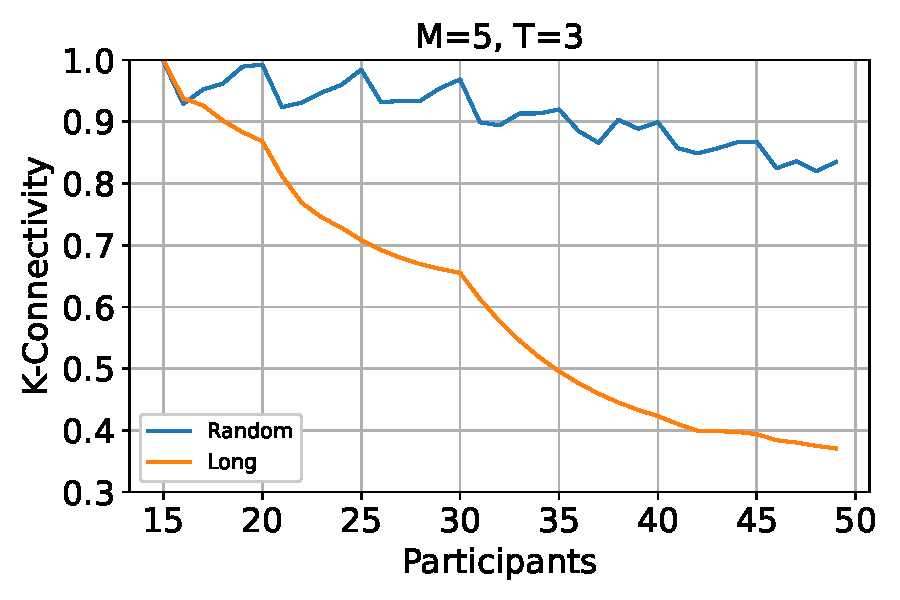
\includegraphics[width=5in]{chapters/figures/NetDelibExp/fig-kcon}
\caption{The k-connectivity of long-path and random-pod network deliberation
networks for $T=3$ stages and a pod size of $M=5$.}
\end{figure}


\section{Experimental Study}
\label{sec:experiment}

\subsection{Experimental Design}

Participants used a pseudonymous online platform (described in Section \ref{sec:exp-platform}) to deliberate on a policy issue.

The deliberation took place asynchronously over a period of 7 days, from Monday, November 15, 2021 through Sunday, November 21, 2021.
The deliberation was divided into 3 rounds of 2--3 days each.
During each round, participants were shown a discussion prompt and were able to post a response to that prompt (Table \ref{tab:prompts}).
Participants were able to view and comment on the posts of other participants assigned to the same pod.
Participants were also able to view posts and comments that were visible to them in previous rounds, but could only interact or reply to posts and comments in the current round.
Before and after each round, participants completed a ranked-choice poll regarding the deliberation topic, allowing the evolution of their preferences to be tracked over the course of the experiment.

\begin{table}
\center
\label{tab:prompts}
\begin{tabular}{|p{0.5in}|p{4.5in}|}
\hline
Stage & Prompt \\
\hline
1 &
Which proposals do you prefer, and why?
If there are disagreements, try asking questions to understand the perspective
of others and to understand the causes of the disagreement.
\\
\hline
2 & In the previous round of discussion, what opinions and reasoning did you
observe in your group?
How much agreement was there?
Were there any disagreements or conflicts?
If so, what were the sources of conflict, and how might they be resolved?
\\
\hline
3 &
What seem to be the most popular opinions?
Do you agree with them?
Has your opinion changed over the course of the discussion?
\\
\hline
\end{tabular}
\caption{Prompts shown to participants during each round of deliberation.}
\end{table}

Participants were recruited from students in an undergraduate university course and received extra credit for participating. 65 participants enrolled and completed at least one round of deliberation.
Basic demographic information was collected and is shown in Table \ref{tab:demographic}.

\begin{table}[]
    \centering
    \begin{tabular}{l l c c}
\hline
\multicolumn{2}{l}{Demographic} & Control & Random-Pod\\
\hline
Age & 18--24 & 30 & 31 \\
& 25--29 & 1 & 0 \\
& 30--34 & 0 & 1 \\
& Non-disclosed & 2 & 0 \\
\hline
Gender & Man & 18 & 14 \\
& Non-binary & 0 & 1 \\
& Woman & 13 & 17 \\
& Non-disclosed & 2 & 0 \\
\hline
Race & Asian & 14 & 16 \\
& Black or African American & 1 & 1 \\
& Hispanic & 1 & 0 \\
& White & 13 & 11 \\
& White, Asian & 1 & 4 \\
& Non-disclosed & 3 & 0 \\
\hline
    \end{tabular}
    \caption{Demographic statistics for experiment participants.}
    \label{tab:demographic}
\end{table}

Participants were assigned to one of two conditions at the time of enrollment.
Assignments were uniformly at random.
Stratified sampling would be preferable in order to ensure even demographic distributions, but was not feasible due to software and time constraints.
However, we manually confirmed that each condition had comparable demographics.
The two conditions were:
\begin{description}
\item[Control]{
Participants in the control condition engaged in conventional deliberation in a single large group.
Posts and comments by participants in the control condition were visible
to all others in the control condition for the duration of the deliberation.}
\item[Random-Pod (Network Deliberation)]{
Participants in this condition were divided into small pods ($\leq 5$ participants).
Posts and comments made by participants in this condition were only visible to others in their current pod.
Participants in this condition were assigned to a new pod at the beginning of each round of deliberation using the random-pod assignment method, producing a structurally efficient communication network.}
\end{description}


\subsection{Deliberation Topic}
The policy issue chosen as the topic of deliberation is a crucial component
of the experiment.
The topic was chosen carefully according to several criteria:
\begin{itemize}
\item Relevant to the experimental population;
\item Amenable to participants changing their preferences based on new information or reasoning;
\item Amenable to a predefined list of proposed solutions;
\item Sufficiently complex to have three or more proposed solutions;
\item Timely, but unlikely to be influenced by current events during the deliberation.
\end{itemize}

Participants were students in a university undergraduate course and deliberated on the topic and format of one section of their final exam.
As the outcome of the final poll determined the content of a real portion of their final exam, participants had an intrinsic incentive to advocate for their true preferences.
The question and alternatives presented to participants were:

\begin{displayquote}

The 2021 [redacted] final exam will include a section worth up to 10\% based on the content covered during the first part of the semester. Which of the following options should be chosen for the topic and format of that section of the exam?

\begin{description}
\item[Prop. 1]{Open-ended with partial credit (2 questions, 5 points each) - Ch. 1-2: Intro to networks.}
\item[Prop. 2]{Open-ended with partial credit (2 questions, 5 points each) - Ch. 3: Bridges, clustering, triadic closure, strong and weak ties, and the Strong Triadic Closure Property.}
\item[Prop. 3]{Multiple choice with no partial credit (5 questions, 2 points each) - Ch. 4: Homophily, selection, social influence, and social-affiliation networks.}
\item[Prop. 4]{Multiple choice with no partial credit (5 questions, 2 points each) - Ch. 5: Signed networks and balance theory.}
\item[Prop. 5]{True/false with no partial credit (10 questions, 1 point each) - Ch. 6: Game theory, best responses, and Dominant Strategies, Nash equilibrium.}
\item[Prop. 6]{True/false with no partial credit (10 questions, 1 point each) - Ch. 9:  Auctions.}
\end{description}
\end{displayquote}


\subsection{Experimental Platform}
\label{sec:exp-platform}

We have modified the free and open-source Loomio platform \cite{jackson_open_2016} to implement network deliberation.
Loomio is a widely-used online deliberation platform which provides both forum functionality (Figure \ref{fig:reply}) and various forms of voting, including ranked-choice (Figure \ref{fig:vote}).
Loomio is popular among worker-owned cooperatives and grassroots organizations (Loomio itself is a worker-owned cooperative).
Loomio was chosen for its combination of built-in functionality, existing user base, and open-source extensibility.

The modified platform implements both random-pod and long-path assignment methods and automatically reassigns participants when the stage is advanced.
In addition to network deliberation features, we have made several modifications used by the experiment.
Upon signing in for the first time, participants are randomly assigned to a treatment condition.
Participants are also assigned an alias which they will use throughout the deliberation (Figure \ref{fig:alias}).

\begin{figure}
\label{fig:reply}
\center
\frame{
\includegraphics[width=5in]{chapters/figures/NetDelibExp/fig-reply.png}}
\caption{Participants can perform standard forum actions, such as posting and commenting.}
\end{figure}

\begin{figure}
\label{fig:vote}
\center
\frame{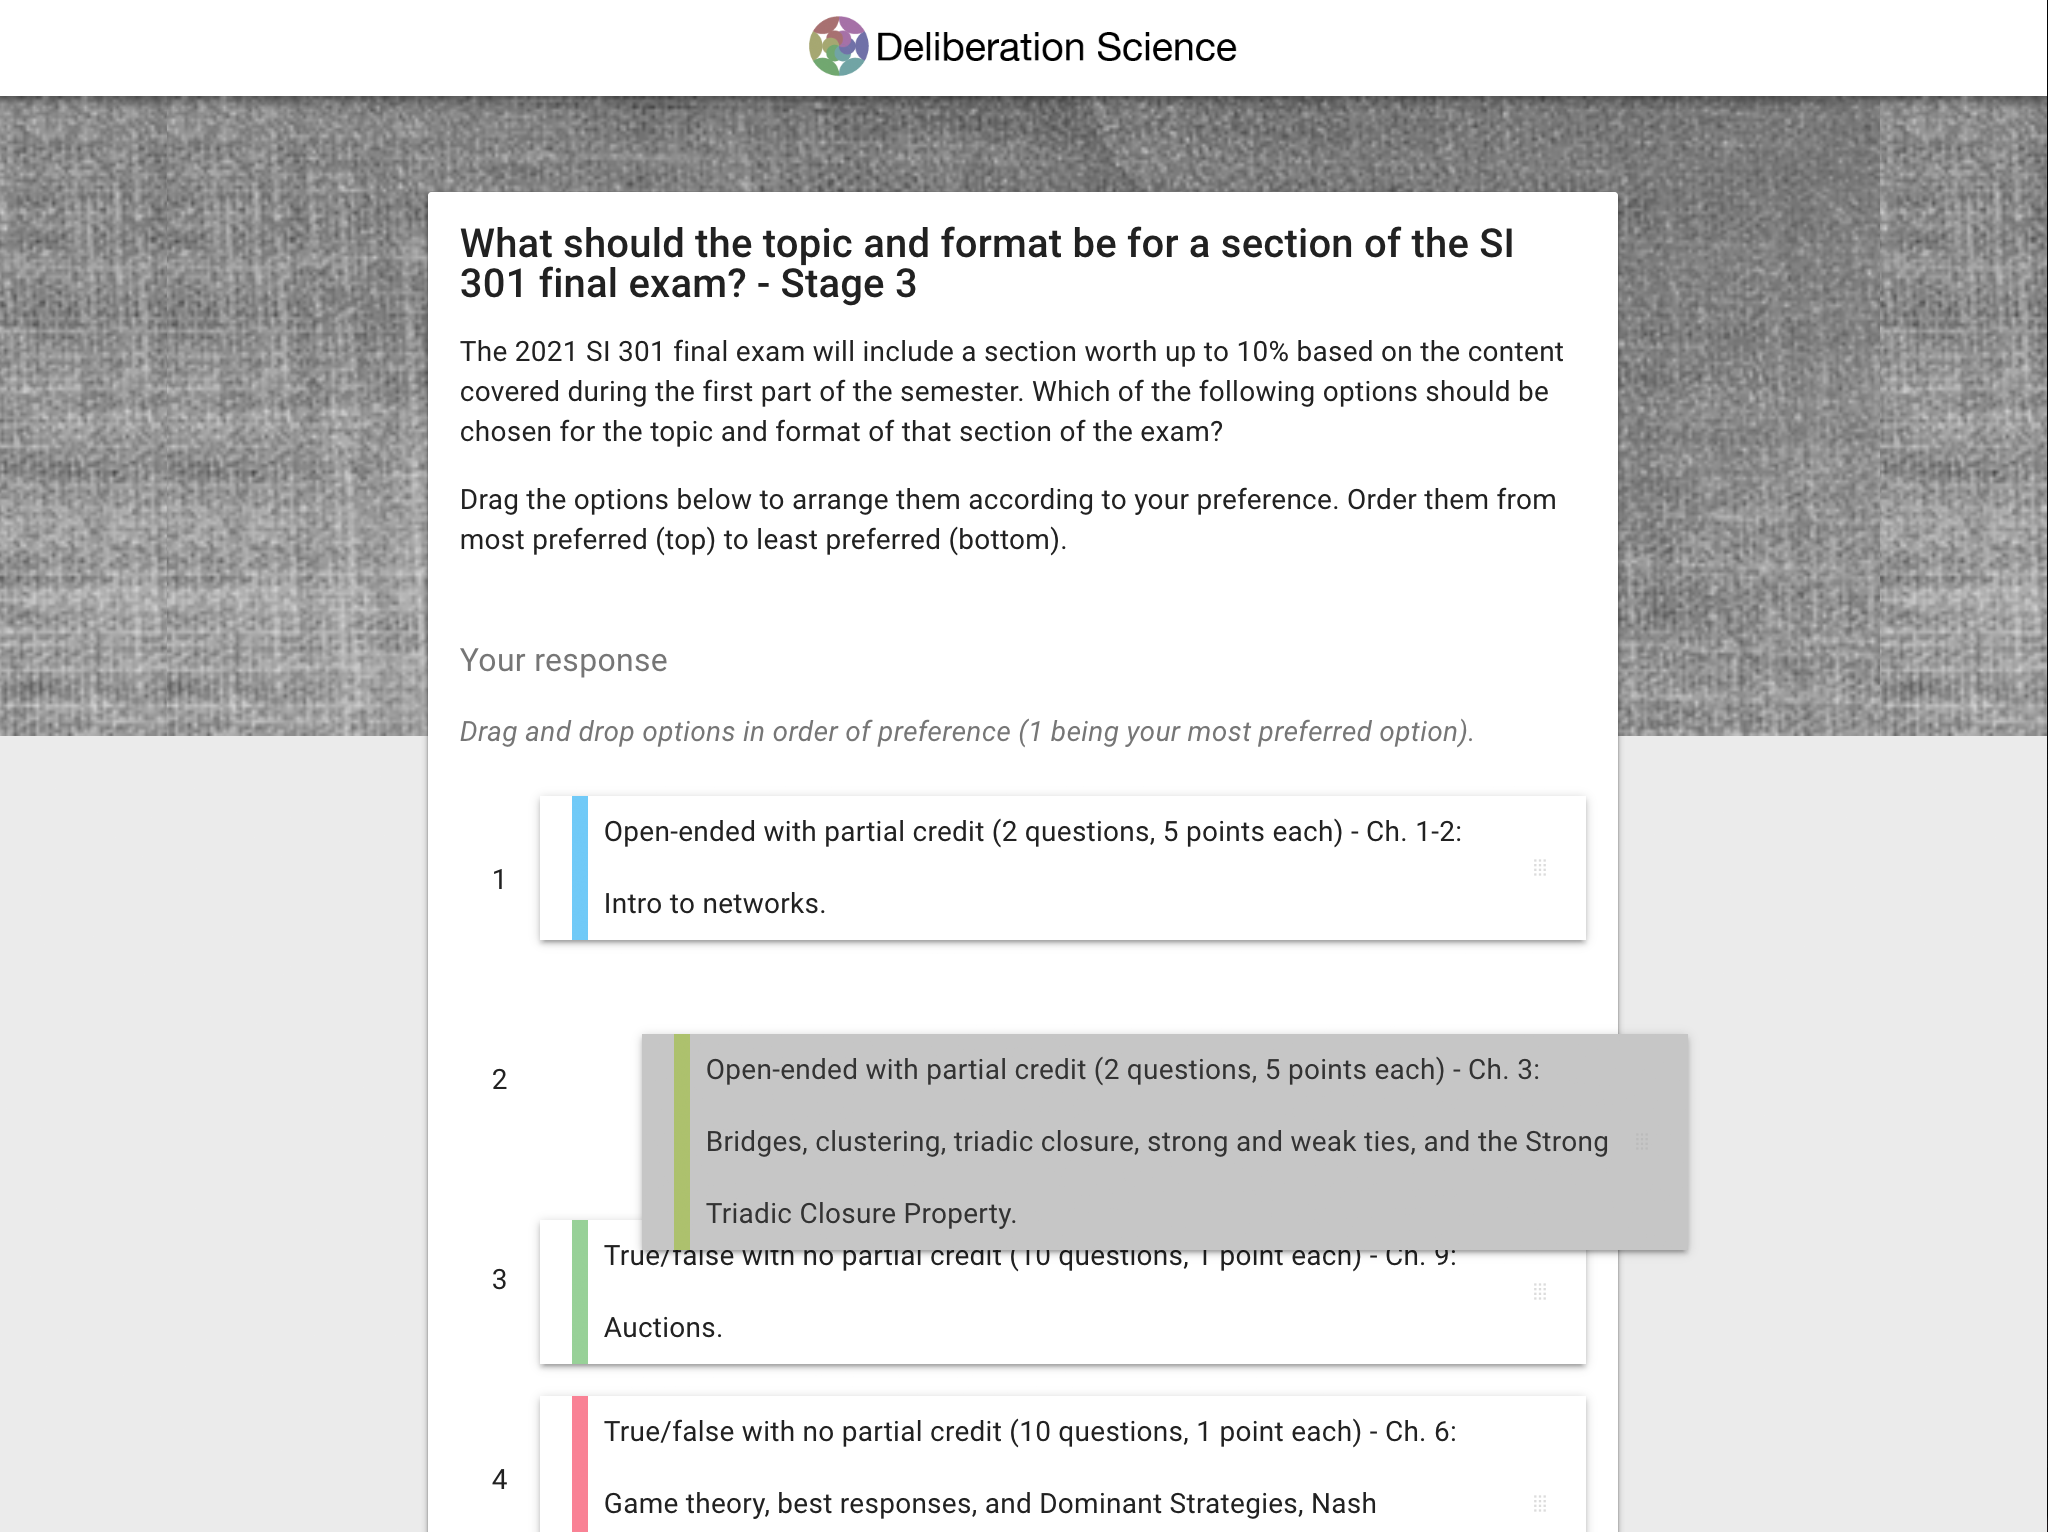
\includegraphics[width=5in]{chapters/figures/NetDelibExp/fig-vote.png}}
\caption{Participants are presented with a ranked-choice voting screen between rounds of deliberation.}
\end{figure}

\begin{figure}
\label{fig:alias}
\center
\frame{
\includegraphics[width=3in]{chapters/figures/NetDelibExp/fig-alias.png}}
\caption{Participants are assigned an alias for the duration of the experiment.}
\end{figure}


\section{Results}
\label{sec:res}

\subsection{Preferences and Outcome}
\label{sec:res-outcome}

We report the outcomes of several voting methods over the course of the deliberation in Table {\ref{tab:outcome} and show the evolution of first-choice vote distributions in Figure \ref{fig:firstplace}.
The pre-deliberation poll shows similar initial preferences across the control and random-pod groups.
A Condorcet winner exists in both groups, and in both cases that winner is Prop. 2.
Prop 2. also claims a plurality of first-choice votes in both groups.
The only notable difference is that in the control group, Prop. 1 wins under the Borda Count method, suggesting that the contest between Props. 1 and 2 are very close and that participants who did not list Prop. 1 in first place still ranked it highly.

\begin{table}[]
    \centering
    \begin{tabular}{c c c c c c c}
\hline
& \multicolumn{3}{c}{Control} & \multicolumn{3}{c}{Random-Pod} \\
\cmidrule(r){1-1}
\cmidrule(lr){2-4}
\cmidrule(l){5-7}
Round & Condorcet & Plurality & Borda &
Condorcet & Plurality & Borda \\
\cmidrule(r){1-1}
\cmidrule(lr){2-4}
\cmidrule(l){5-7}

0 & prop2 & prop2 & prop1 & 
prop2 & prop2 & prop2 \\

1 & prop1 & prop1 & prop1 &
prop2 & prop2 & prop2 \\

2 & prop1 & prop1/prop2 & prop1 &
prop2 & prop2 & prop2 \\

3 & prop1 & prop1 & prop1 &
prop2 & prop2 & prop2 \\
\hline
    \end{tabular}
    \caption{Referendum outcome after each round of deliberation (initial=0).}
    \label{tab:outcome}
\end{table}

\begin{figure}
    \centering
    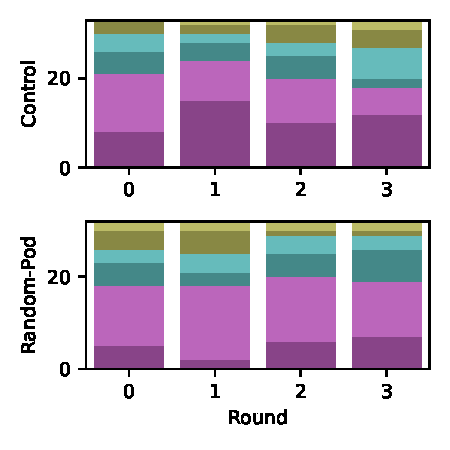
\includegraphics[width=3in]{chapters/figures/NetDelibExp/fig-counts.pdf}
    \caption{Number of first-choice votes for each alternative over the course of the deliberation.}
    \label{fig:firstplace}
\end{figure}

Over the course of the deliberation, the preference profiles of the control and random-pod groups show notable differences.
In the control group, Prop. 1 becomes the Condorcet winner after round 1 and wins across all other voting methods.
Prop 1. remains the winner in the control group throughout the rest of the deliberation, with one exception: Prop. 1 and Prop. 2 tie for plurality voting in round 2.
In the random-pod group, Prop. 2 remains the winner across all voting methods throughout the entire deliberation.
We compare participants' preferences before and after the deliberation in Figure \ref{fig:countmatrix}.
The most striking feature is that a number of participants (4) in the control group who initially ranked Prop. 2 highest then went on to rank Prop 1. the highest in the final poll.
These participants are a significant driver of the switch from Prop 2. to Prop 1. in the control group.
While the random-pod group does show some participants switching away from Prop. 2, those participants shift to the less popular Props. 3 and 4 rather than Prop 1.
In the sections that follow, we will further analyze the evolution of participant preferneces and the potential mechanisms driving them.

\begin{figure}
    \centering
    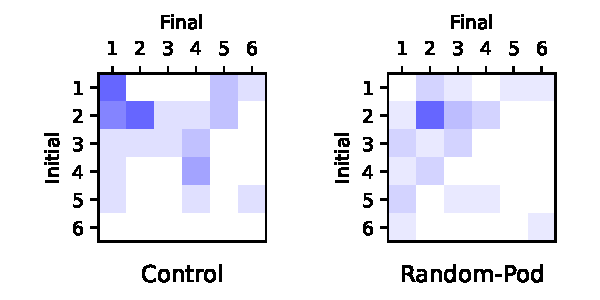
\includegraphics[width=4in]{chapters/figures/NetDelibExp/fig-count-matrix.pdf}
    \caption{Histogram of participants' initial (row) and final (column) first-choice votes.}
    \label{fig:countmatrix}
\end{figure}


\subsection{Activity}
\label{sec:res-activity}

Here we describe the trends we observe in participants' deliberation activity and the potential impact on participant preferences.
Overall, the nubmer of comments per participant shows a heavy-tailed distribution (Figure \ref{fig:commentcounts}) with a mode of one comment per participant.
The random-pod group shows less of a heavy-tail, with more participants posting a single comment per round and a smaller maximum count (2--3 comments vs. 3--4 for control).
The random-pod group thus shows a more equal division of activity across participants.

\begin{figure}
    \centering
    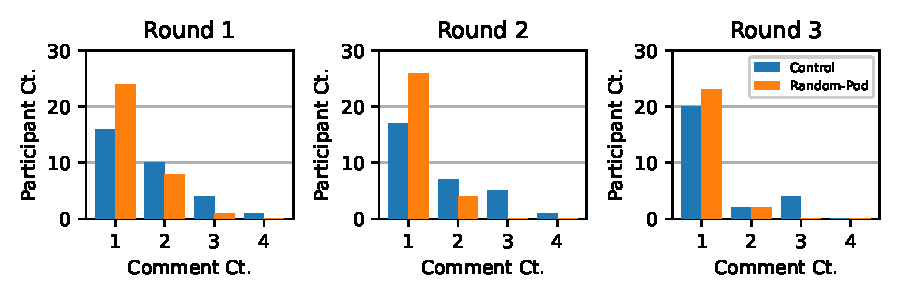
\includegraphics[width=6in]{chapters/figures/NetDelibExp/fig-comment-counts.pdf}
    \caption{Histogram of the number of posts made by participants during each round of deliberation.}
    \label{fig:commentcounts}
\end{figure}

Figure \ref{fig:commentrounds} shows the comment counts for each round as well as the Shannon entropy of participant comment counts.
The random-pod group shows a lower total number of comments and a higher entropy, again showing a more equal division of activity across participants.

\begin{figure}
    \centering
    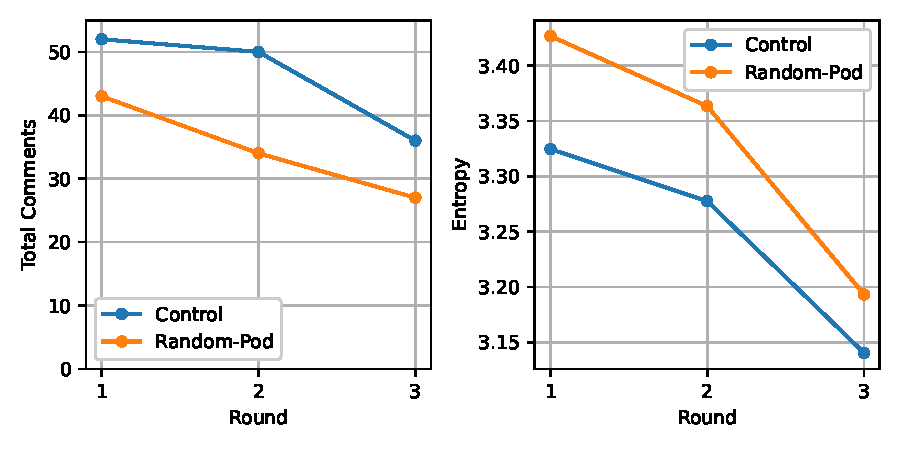
\includegraphics[width=6in]{chapters/figures/NetDelibExp/fig-comment-rounds.pdf}
    \caption{The total number of comments in each round (left) and the Shannon entropy of participant comment counts (right).}
    \label{fig:commentrounds}
\end{figure}

The more equal distribution of comments in the random-pod group is consistent with our expectation that network deliberation promotes equal participation.
The reduction in overall participation is also notable and suggests low participation as a potential consideration in network deliberation settings.


\subsection{Deliberation Content}
\label{sec:res-content}

The content of participant comments gives additional insight into how preferences were infuenced by deliberation.
We pay special attention to comments pertaining to the two most popular alternatives: Props. 1 and 2.
Preferences for these alternatives evolved differently between the control and random-pod groups.

Comments across both groups frequently advocated for Props. 1 and 2 without specifying a preference between the two:
\begin{displayquote}
P09: Opened ended questions allow for partial credit while multiple choice and true false has no partial credit. I feel comfortable with chapters 1, 2, and 3 [Props. 1 \& 2] as they are the easiest. I am least comfortable with auctions [Prop. 6].
\end{displayquote}
However, some participants advocated for one or the other:
\begin{displayquote}
P64: I think Intro to Networks [Prop. 1] should be chosen. I like the open ended question format of this, as it allows for partial credit. In addition to this, since these were the topics that were taught in the beginning they provide a base of everything we have learned in the class and as a result I think this material would be very helpful for it to be covered on our final exam.
\end{displayquote}
\begin{displayquote}
P10: I prefer the open-ended questions on chapter 3 [Prop. 2] because I feel like many of these types of questions would have several requirements, so it is very possible to receive partial credit if you partially understand. The main reason I choose chapter 3 [Prop. 2] over chapters 1/2 [Prop. 1] is because I don't know what questions from chapters 1/2 [Prop. 1] would look like, and I know how to prepare for chapter 3 [Prop. 2].
\end{displayquote}
While in the minority, some participants advocated for other proposals:
\begin{displayquote}
P43: I think the topics covered in chapter 6 [Prop. 5] should definitely be on the final. I'm personally indifferent between true/false.
\end{displayquote}


\subsection{Preference Evolution}

As shown in Table \ref{tab:outcome} and Figure \ref{fig:firstplace}, both groups initially preferred Prop. 1, with the control group switching to Prop. 2 after round 1 while the random-pod group maintained its initial preference.
We now analyze participant preferences and their evolution in more detail.

\subsubsection{Agreement}
\label{sec:res-agreement}

\begin{figure}
    \centering
    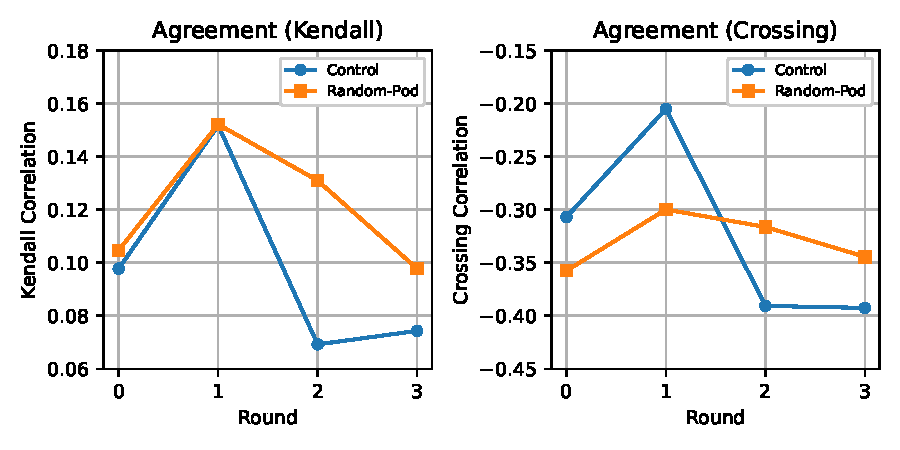
\includegraphics[width=6in]{chapters/figures/NetDelibExp/fig-agreement-fillattr.pdf}
    \caption{Treatment-level agreement over the course of the deliberation. Agreement is calculated as the mean pairwise correlation between participants using either Kendall corellation (left) or weighted crossing correlation (right).}
    \label{fig:agreement}
\end{figure}

We report the intra-group agreement throughout the course of the deliberation in Figure \ref{fig:agreement}.
We calculate agreement using both the Kendall correlation
and the weighted crossing correlation.
The Kendall correlation is commonly used in social choice and weights contributions from each rank equally.
The weighted crossing correlation places a higher weight on
higher-ranked preferences.
In both cases, the avarage pairwise agreement follows similar a similar pattern.
Both the control and random-pod groups show an increase in agreement after the first round of deliberation,
followed by a decrease.
In the control group, the decrase is more rapid and more extreme than in the random-pod group.
Using weighted crossing agreement, the difference-in-differences between control and random-pod groups is 0.68, noting that weighted crossing ranges from -1 to +1.

Our results show that in our experiment, the random-pod group 
experienced a small but robust increase in agreement,
wile the control group experienced a sharp increase followed by an even sharper decrease.
These results support the hypothesis H1 that network deliberation contributes to increased agreement relative to conventional single-group deliberation.
However, this effect is due more to a decrease in agreement
within the control group than an increase in the random-pod group.
After an initial increase in agreement, both groups showed an unexpected ``rebound'' effect.
In the control group, this rebound resulted in a net reduction in agreement, suggesting the presence of negative social influence.

\subsubsection{First-Choice Votes}
\label{sec:res-firstchoice}

\begin{figure}
    \centering
    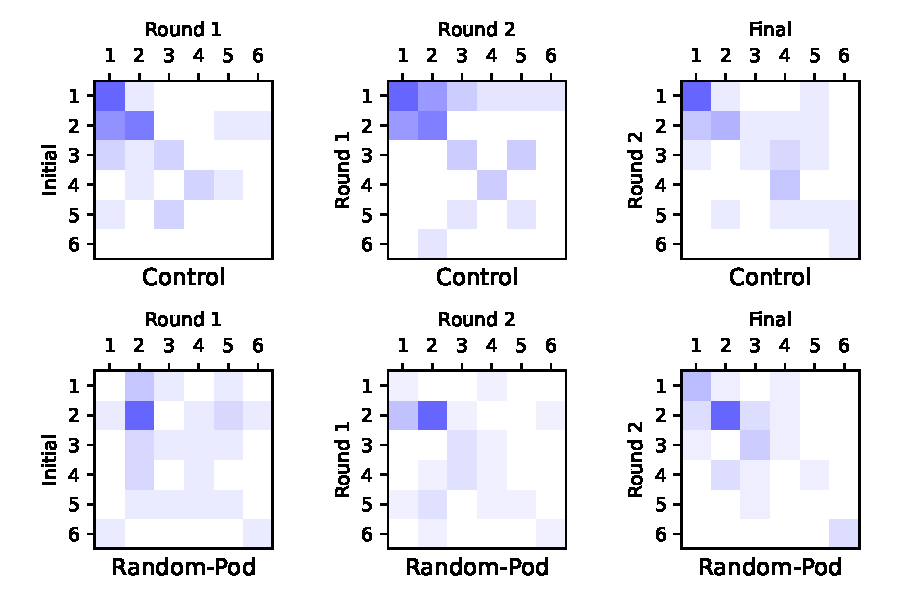
\includegraphics[width=6in]{chapters/figures/NetDelibExp/fig-round-matrix.pdf}
    \caption{Histograms of participants' first-choice votes before and after each round.}
    \label{fig:roundmatrix}
\end{figure}

By focusing on first-choice votes and on the most popular alternatives (Props. 1 \& 2), we can offer some insight into the differences in preference evolution we observe between the control and random-pod groups.
Figure \ref{fig:roundmatrix} shows the evolution of first-choice preferences over the course of each round of deliberation.
Initially, the control and random-pod groups had similar distributions of first-chioce votes for Props. 1 \& 2, with both clearly favoring Prop. 2 (13:8 for control and 13:5 for random-pod).
However, first-round comments regarding these two proposals differed substantially between the two groups.
In the control group, a majority of comments (7:2) favored Prop. 1 while in the random-pod group, a majority favored Prop. 2 (9:2).
Remarkably, the support expressed for Prop. 1 by the control group during round 1 was counter to the group's initial preference for Prop. 2.
After that round however, a majority of control group participants reported a first-choice preference for Prop. 1 over Prop. 2 (15:9).
In the random-pod group, Prop. 2 remained the most popular and received an even higher share of first-choice votes (16:2) after round 1.

In both the control and random-pod groups, we see round 1 deliberation clearly favoring one alternative, which then gains a number of first-choice votes, suggesting social influence.
This social influence is further evidenced by the increase in agreement observed for both groups over the course round 1 (Figure \ref{fig:agreement}).

The control group varies from the random-pod group in that the round 1 advocacy and subsequent preference shifts are opposite to the original preferences.
In other words, there is evidence of an information cascade flipping the control group's preference from Prop. 2 to Prop. 1 over the course of round 1.
While many factors contribute to the formation of an information cascade, we suggest that network deliberation structure of the random-pod group may have reduced the liklihood of such a cascade in that group.
The pod structure limits how many participants can be exposed to influence from any particular individual during a single round.
Furthermore, the more even distribution of participation observed in the random-pod group provides participants with more accurate information on the preference distribution of ther peers.
The discussion is less skewed towards highly-vocal participants.

In rounds 2 and 3, the preferences for Props. 1 \& 2 continued to evolve differently for the control and random-pod groups (Figure \ref{fig:roundmatrix}).
In both cases, participants partially reverted towards their initial preferences.
In the control group, particularly during round 2, Prop 1. lost many of its round 1 gains to Props. 3--6, although it still remained the most popular first-choice vote,
and Prop 2. retained a sizeable minority of first-choice votes.
As a result, the control group exhibited a divergence of preferences after round 2, contributing to the drop in agreement seen in Figure \ref{fig:agreement}.
In the random-pod group, many of the participants who had switched from Prop. 1 to Prop 2. after round 1 switched back,
partially reverting the winning margin of Prop 2. towards its original value and contributing to a reduction in agreement.
However, the observed drop in agreement values can't be explained by first-choice votes alone.
The two groups show similar distributions of first-choice vote counts (although assigned to different alterantives) but a notably different level of overall agreement.

\subsection{Social Influence}
\label{sec:res-socialinfluence}

\begin{figure}
    \centering
    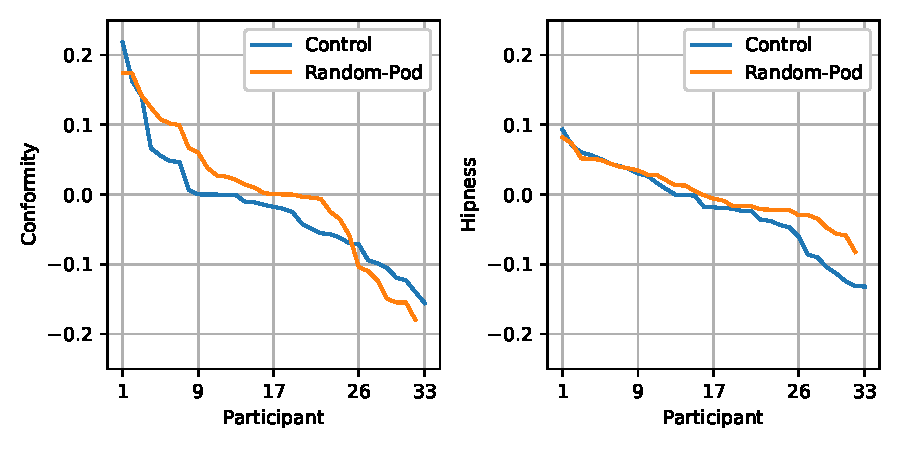
\includegraphics[width=6in]{chapters/figures/NetDelibExp/fig-hipness-conformity.pdf}
    \caption{Conformity and hipness by participant, calculated using initial and final preferences. Values are sorted in descending order for ease of comparison.}
    \label{fig:conformity}
\end{figure}

To better understand the role of social influence in the evolution of preferences, we report the conformity and hipness distributions in Figure \ref{fig:conformity}.
Summing either of these quantities over all participants yields the overall change in mean agreement: -0.597 for control and +0.049 for random-pod.

In the control group, the participants with negative conformity outnumber those with positive conformity:
more participants moved away from others' preferences than toward them, resulting in a negative shift in agreement.
In the random-pod network deliberation group, the number of participants with positive conformity is slightly larger than the number with negative conformity, leading to a slightly positive change in agreement.
The difference between the two groups is most pronounced among small magnitude conformity participants: those who did not change their preferences much over the deliberation.

Alternatively, we can analyze the change in agreement in terms of hipness. The negative change in agreement in the control group can be attributed primarily to a small number of participants with highly-negative hipness.
These participants did not change their preferences much over the course
of the deliberation,
but other participants' preferences moved away from theirs considerably.
Among participants in the random-pod network deliberation group,
those with negative hipness have a notably smaller magnitude,
resulting in more agreement.

\subsubsection{Dynamics of Social Influence}
\label{sec:res-dynamics}

\begin{figure}
    \centering
    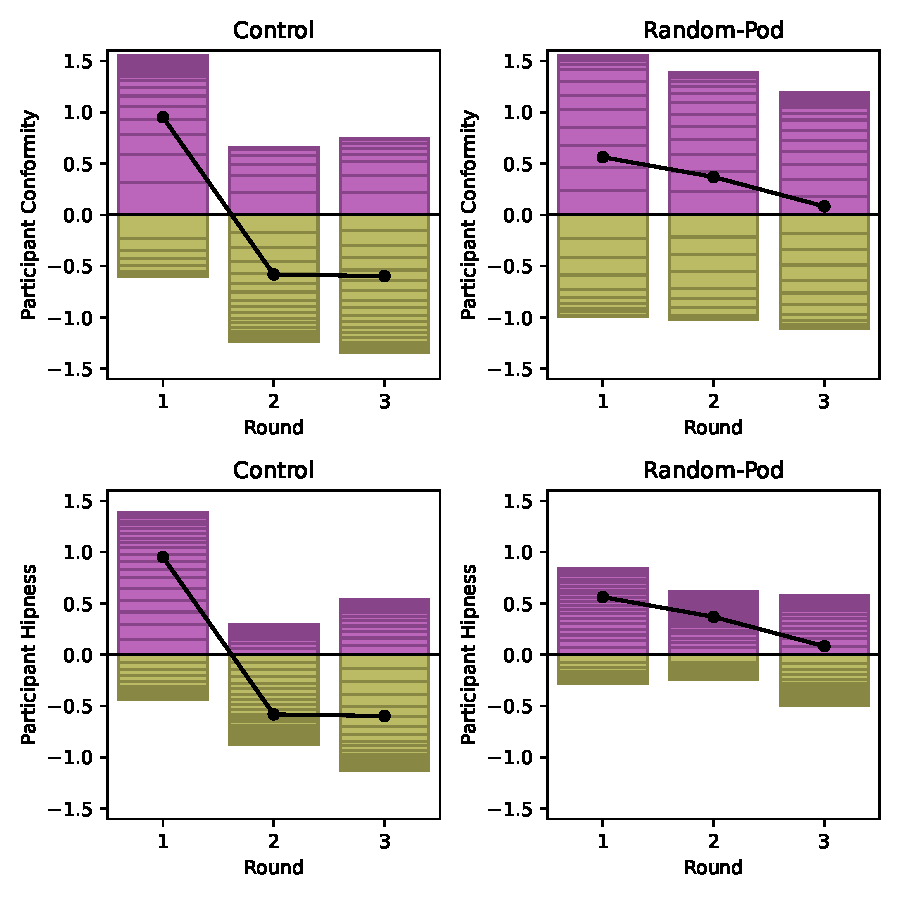
\includegraphics[width=6in]{chapters/figures/NetDelibExp/fig-influence-bar.pdf}
    \caption{Participant contributions to conformity and hipness at each round.}
    \label{fig:influence-bar}
\end{figure}

Figure \ref{fig:influence-bar} shows the conformity and hipness contributions of individual participants after each round
(relative to initial preferences).
The sum of positive and negative contributions (equivalent to the mean difference in agreement) is overlaid.
In the control group, conformity begins mostly positive and high-magnitude after the first round, but switches to mostly negative in subsequent rounds.
In contrast, the random-pod group shows a combination of positive and negative conformity throughout the experiment, with positive conformity maintaining a small majority.
These observations suggest that participants in the control group first conformed towards initially popular preferences, but shifted away from them after the second round of deliberation.
While in the random-pod group, participants showed diverse changes in perference with some convergence towards initially-popular preferences.

Analyzing hipness suggests a similar picture.
The control group shows overwhelmingly positive hipness after round 1, with a switch to primarily negative hipness in subsequent stages.
The random-pod group shows primarily positive hipness throughout most of the experiment, although both positive and negative values are small in magnitude.
So in the control group, changes in preference are divided unevenly between participants.
At first, these changes conform towards the more fixed participants, but after round 2 diverge away from them.
In constrast, within the random-pod group, changes in preference are distributed more evenly and consistently converge towards the more fixed participants.

\subsubsection{Interpretation of Social Influence}
\label{sec:res-interpretation}

Combining the above insights from conformity and hipness measures suggests the following.
The negative shift in agreement in the control group is due
to a majority of participants shifting their preferences away (negative conformity) from a samll number of stubborn participants (highly-negative hipness) without converging on an alternative (lack of positive conformity).
Furthermore, this shift occurs after round 2, following an initial stage of high-conformity.
The random-pod participants also exhibit stubborn participants, but fewer and with smaller magnitude,
and the the majority of participants converge toward each other's preferences (positive conformity).

Our findings show that the random-pod network deliberation group experienced a positive change in agreement relative to the conventional deliberation control group.
The above analysis of individual preference shifts suggests that the decreased agreement in the control group is due to social influence leading a number of participants to shift from more popular preferences to a divergent set of less popular preferences.

\subsection{Survey}

\begin{figure}
    \centering
    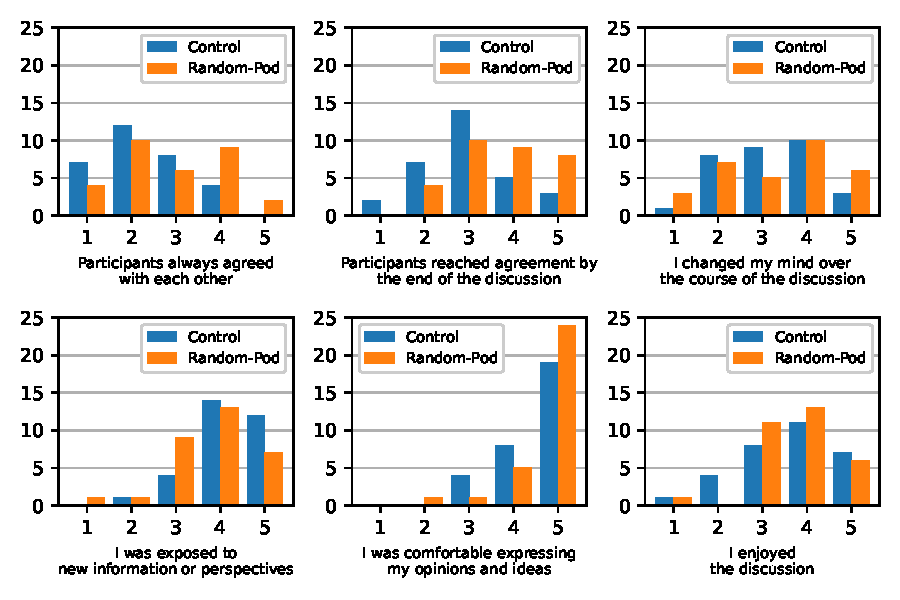
\includegraphics[width=6in]{chapters/figures/NetDelibExp/fig-survey.pdf}
    \caption{Participant post-experiment survey responses on a 5-point Likert scale.}
    \label{fig:survey}
\end{figure}

\begin{table}[]
    \small
    \centering
    \begin{tabular}{l c c c}
\hline
Question & \multicolumn{2}{c}{Median} & p \\
\cmidrule(lr){2-3}
& Control & Random-Pod & \\
\hline
Q1: Participants always agreed with each other
& 2 & 3 & 0.070 \\
Q2: Participants reached agreement by the end of the discussion
& 3 & 4 & 0.015 \\
Q3: I changed my mind over the course of the discussion
& 3 & 4 & 0.663 \\
Q4: I was exposed to new information or perspectives
& 4 & 4 & 0.068 \\
Q5: I was comfortable expressing my opinions and ideas
& 5 & 5 & 0.181 \\
Q6: I enjoyed the discussion
& 4 & 4 & 0.722 \\
\hline
    \end{tabular}
    \caption{Median responses for post-experiment survey (5-point Likert scale). Reported p values are for a two-sided Mann-Whitney test. The Šidák correction places the threshold at $p < 0.0085$ for a FWER of less than $\alpha=0.05$.}
    \label{tab:survey}
\end{table}

The results of the post-experiment survey are shown in Table \ref{tab:survey} and Figure \ref{fig:survey}.
After correcting for multiple comparisons using the Šidák correction, the Mann-Whitney test finds no significant difference between the control and random-pod groups.
However the observed differences (and lack of differences) in median suggest a starting point for future work.
We expected the random-pod group to be better at identifying and resolving disagreements, which would result in a lower score for Q1 and a higher score for Q2.
Instead, we observe a higher median score for both.
Given that initial preference profiles were similar for the two groups, the lower perception of agreement in the control group could be driven by a number of mechanisms, such as higher visibility of disagreements or polarization over the course of the deliberation.
The difference in perceptions of agreement across conventional and network deliberation could be a fruitful area for future research.

\section{Discussion}
\label{sec:discussion}

We hypothesized (H1) that network deliberation tends to reach a higher level of agreement than conventional single-group deliberation.
The observed agreement calculated from polls throughout the experiment experiment supports this hypothesis (Section \ref{sec:res-agreement}).
However, our hypothesis was based on the assumption that network deliberation would more effectively identify and resolve disagreements,
leading us to expect a large increase increase in agreement in the random-pod group.
Instead, we observe a small increase of agreement within the random-pod group and a large decrease within the control group.
So while we do see more of an improvement in agreement under network deliberation, our observations are more consistent with a protective effect against a disagreement-producing mechanism, than with the originally hypothesized agreement-producing mechanism.

We also sought to understand how preferences evolve during network deliberation vs. conventional deliberation (RQ1).
We focused our analysis on first-choice votes in particular (Section \ref{sec:res-firstchoice}).
We also quantified the observed social influence throughout the experiment (Section \ref{sec:res-dynamics}).
In both the control and random-pod group, we observed preferences shifting in favor of alternatives that received overwhelming support in round 1 deliberation comments.
These comments were consistent with initial preferences in the random-pod group, but counter to initial preferences in the control group.
An information cascade, in which participants conformed to a less popular opinion believing it to be more popular, is one likely mechanism.
The skewed distribution of activity in the control group (Section \ref{sec:res-activity}), as well as the large number of negative-conformity participants (Section \ref{sec:res-socialinfluence}) are both consistent with an information cascade in the control group.
In network deliberation, participants are limited to interacting with others in the same pod, creating a barrier to the spread of information cascades.
Thus, the network deliberation structure may explain why round 1 comments in the random-pod group were consistent with initial preferences, i.e., did not show evidence of an information cascade.

It is interesting to note that while the control group showed considerable positive conformity in round 1, most participants switched to negative conformity in later rounds, while in the random-pod group, positive conformity was relatively consistent.
In other words, the preferences of the control group converged in round 1, but diverged in later rounds, resulting in the observed sharp drop in agreement (Figure \ref{fig:influence-bar}).
As nothing changed in the control group between the first and subsequent rounds, it is interesting to consider why the conformity switched from mostly positive to mostly negative, e.g., why preferences diverged during round 2 after converging in round 1.
Possible explanations include a ``rebound'' effect from an information cascade or a time-dependent effect only emerging in later rounds.

Motivated by prior literature identifying conflict discovery and resolution as a benefit of participatory decision-making, we also considered the effect of network deliberation on conflict resolution (RQ2).
Unexpectedly, we found that the random-pod group provided only a small increase in agreement, but that the control group actually produced disagreement by the end of the deliberation.
Interestingly, the first-choice votes show a similar level of agreement in the two groups, so the control group disagreement is largely due to second-choice votes and below.
One possible explanation is that participants disagreeing on first-place votes became more polarized against each other, lowering each other's top-choice in their own preferences, but additional research is necessary to test this hypothesis.

We note that in this experiment, the skewed distribution of participation in the control group acted to amplify proponents of a minority preference, which later became the majority preference in a possible information cascade.
However, a skewed distribution of participation could potentially have the opposite effect of further amplifying an already majority preferences and overshadowing minority preferences.
A better understanding of the factors determining which preferences are amplified would contribute to an understanding of when network deliberation is preferable to conventional.

We also note that the overall level of participation was lower in the random-pod group, very likely due to the smaller group size.
The low level of activity could be one factor contributing to the lack of conflict identification in the random-pod group.
It is thus desirable to better understand how factors including group size contribute to activity level.


\section{Conclusion}
\label{sec:ch04conclusion}

We have reported the results of a controlled experiment comparing an efficient network deliberation network to conventional single-group deliberation.
We found that network deliberation produced a more positive change in agreement consistent with our hypothesis. However, we found that this change was due primarily to a decrease in agreement in the conventional group, suggesting a mechanism that protects against disagreement rather than facilitating agreement.
We find evidence of an information cascade in the conventional group strong enough to alter the Condorcet winner.
Our findings suggest that protection against information cascades may be one mechanism underlying the success of network deliberation in large-scale collaborations.

